% ==============================================================================
% SECCION 4: RESULTADOS
% ==============================================================================
\section{Resultados}\label{sec:resultados}

\subsection{Resultados de Identificación Experimental en Banco}\label{subsec:res_identificacion}

\begin{figure*}[!t]
    \centering
    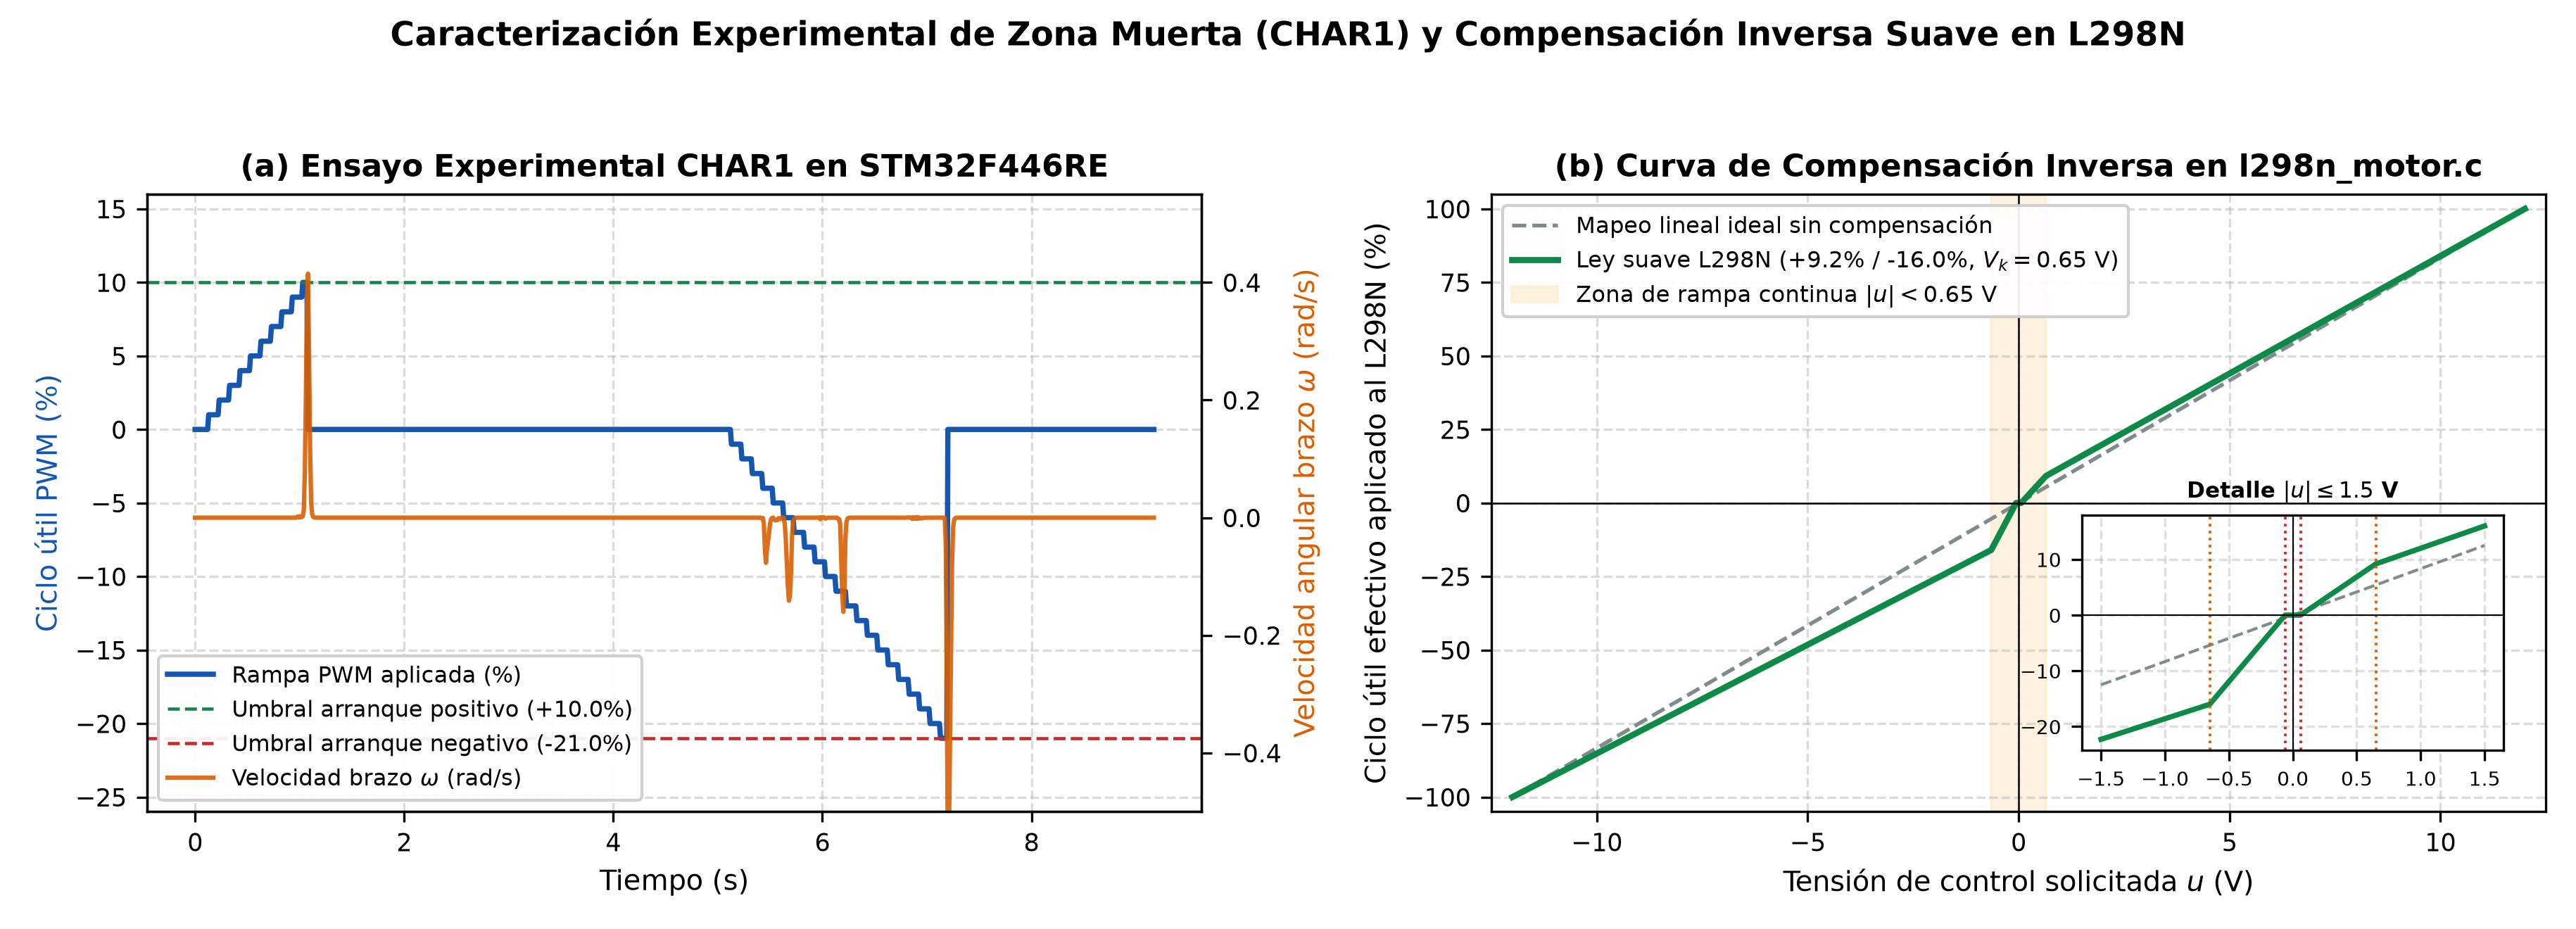
\includegraphics[width=0.78\textwidth]{fig_exp_zona_muerta_y_l298n.png}
    \caption{Resultados experimentales del ensayo \texttt{CHAR1} ($n=918$ muestras, \qty{9.17}{\second}): respuesta angular y velocidad del brazo ante rampa de ciclo útil con umbrales de ruptura estática en $+10.0\%$~PWM CCW y $-21.0\%$~PWM CW (a), y comparación entre la respuesta estática medida y la curva compensadora continua por tramos implementada (b).}
    \label{fig:exp_zona_muerta}
\end{figure*}

\begin{figure*}[!t]
    \centering
    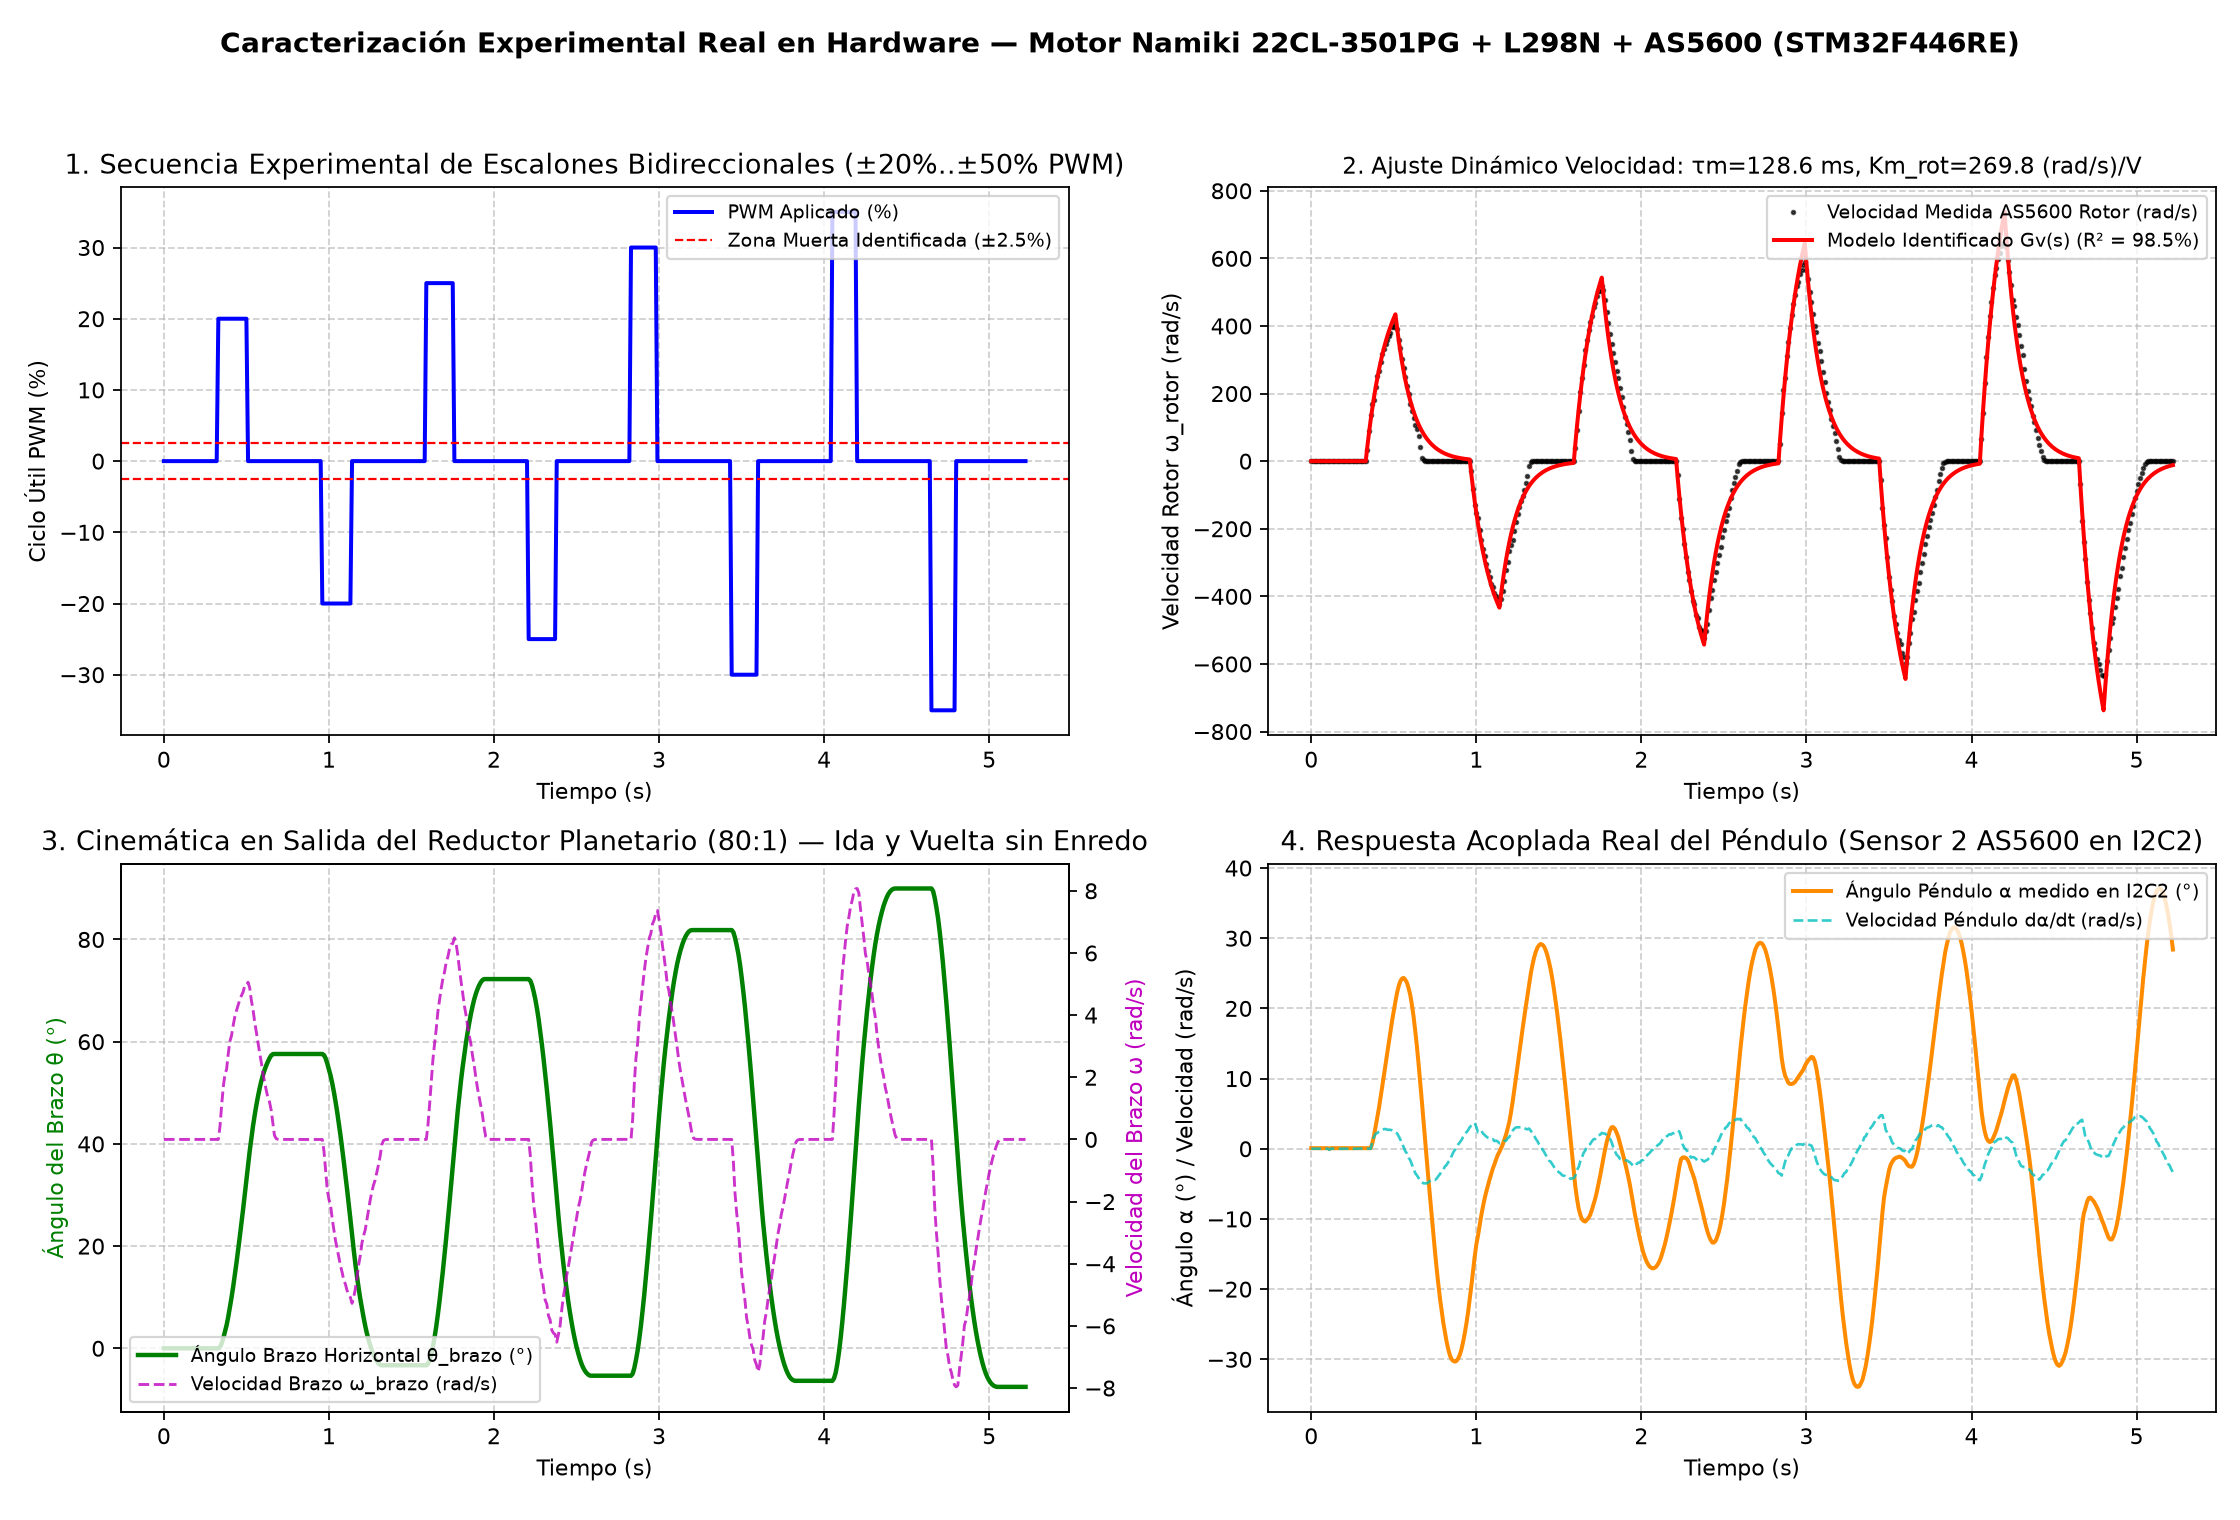
\includegraphics[width=0.69\textwidth]{fig_exp_caracterizacion_motor.png}
    \caption{Resultados experimentales del ensayo \texttt{CHAR2} ($n=538$ muestras, \qty{5.37}{\second}): excitación mediante ocho escalones bidireccionales de tensión y superposición entre la velocidad medida del brazo $\dot{\theta}(t)$ y la respuesta temporal del modelo lineal identificado de primer orden ($R^2 = 98.51\%$, $\mathrm{NRMSE} = 87.79\%$).}
    \label{fig:exp_motor}
\end{figure*}

\begin{figure*}[!t]
    \centering
    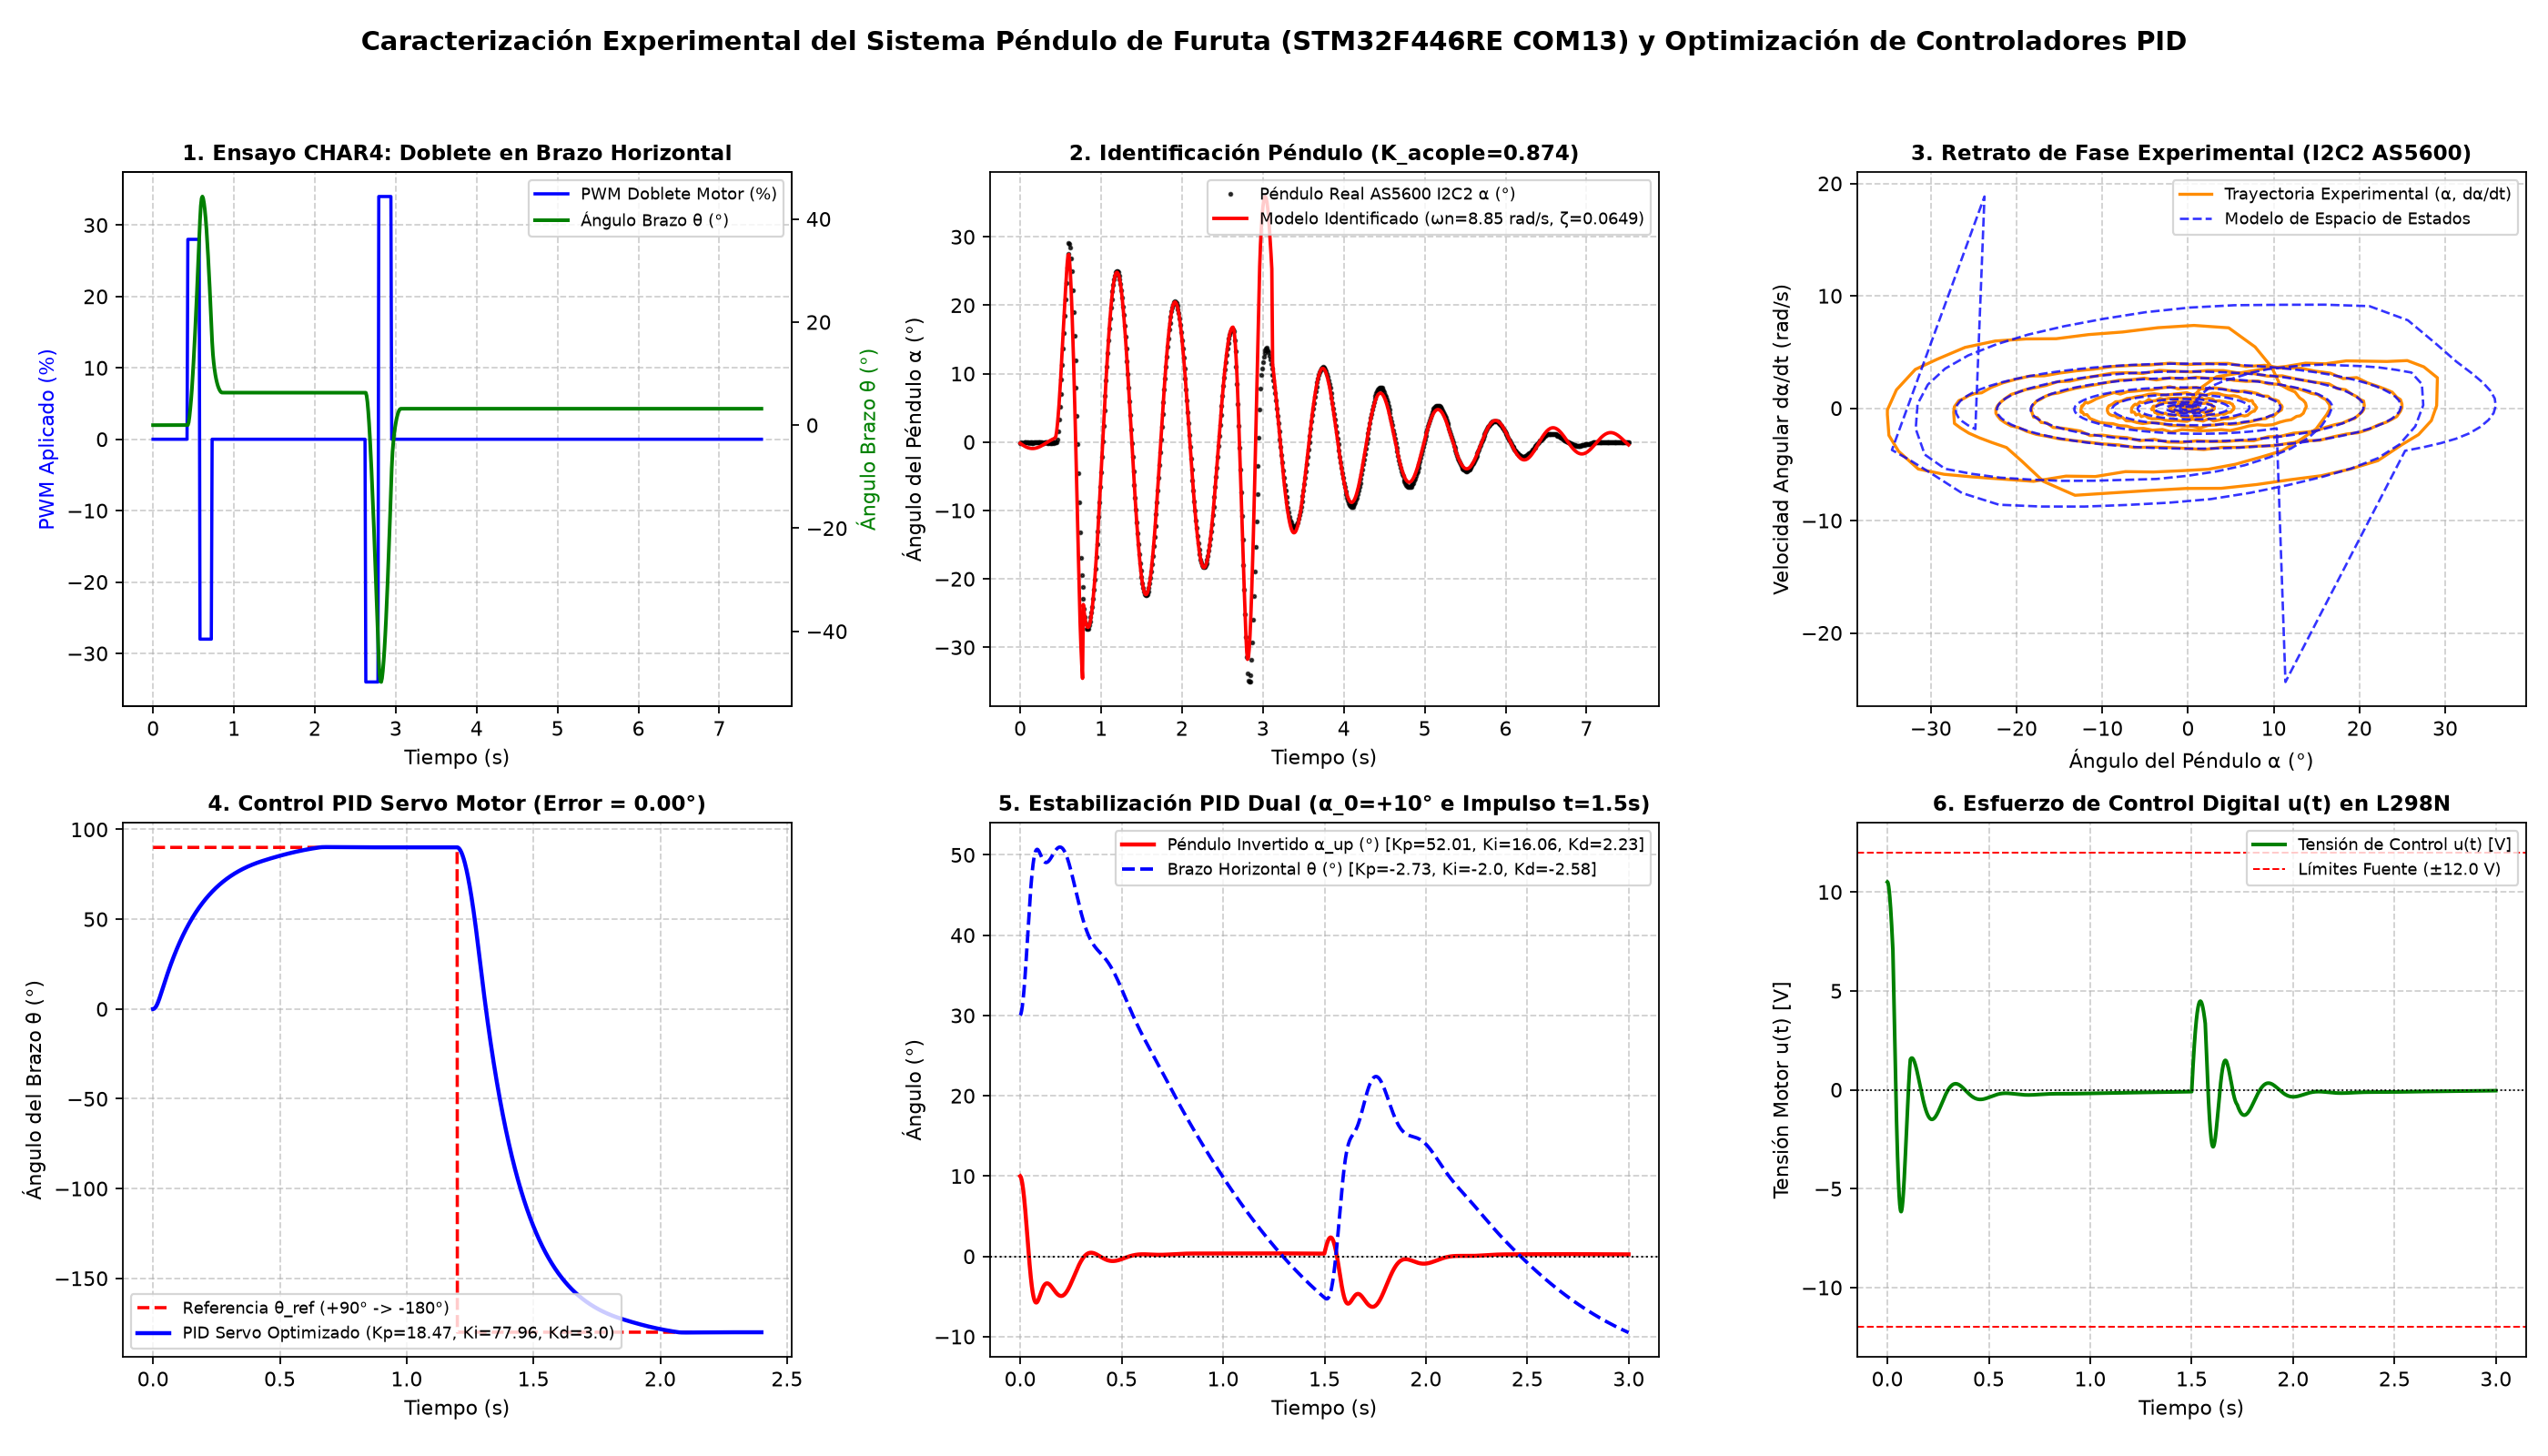
\includegraphics[width=0.74\textwidth]{fig_exp_caracterizacion_sistema.png}
    \caption{Resultados experimentales del ensayo acoplado \texttt{CHAR4} ($n=768$ muestras, \qty{7.67}{\second}): respuesta ante dobletes bipolares de excitación y ventanas de decaimiento libre con freno electromagnético activo, superponiendo la trayectoria pendular medida $\alpha(t)$ con el modelo acoplado y el ajuste de fricción mixta viscosa--Coulomb ($R^2 = 99.64\%$).}
    \label{fig:exp_sistema}
\end{figure*}

En la Fig.~\ref{fig:exp_zona_muerta} se presentan los registros obtenidos durante la prueba de rampa de ruptura estática \texttt{CHAR1} ($n=918$ muestras, duración de \qty{9.17}{\second}). En la rama positiva en sentido antihorario (CCW), el inicio del movimiento del brazo se registró en un ciclo útil de $+10.0\%$~PWM, equivalente a una tensión umbral de $+\qty{1.20}{\volt}$. En la rama negativa en sentido horario (CW), el umbral de ruptura estática se midió en $-21.0\%$~PWM, correspondiente a $-\qty{2.52}{\volt}$. Una vez superado el reposo inicial, el umbral dinámico de sostenimiento de giro se ubicó en $2.5\%$~PWM ($\qty{0.30}{\volt}$). En la Fig.~\ref{fig:exp_zona_muerta}(b) se contrasta el perfil experimental frente a la ley compensadora continua~\eqref{eq:comp_l298n} configurada con valores de arranque $\mathrm{dz}^+=9.2\%$~PWM y $\mathrm{dz}^-=16.0\%$~PWM, banda silenciosa central de $\qty{0.06}{\volt}$ y tensión de rodilla $V_k=\qty{0.65}{\volt}$.

Los resultados de la identificación dinámica del actuador mediante el ensayo \texttt{CHAR2} ($n=538$ muestras, \qty{5.37}{\second}) se muestran en la Fig.~\ref{fig:exp_motor}. El ajuste por mínimos cuadrados no lineales sobre la secuencia de ocho escalones bidireccionales arrojó una ganancia estática del brazo $K_v=\qty{3.3720}{(\radian\per\second)\per\volt}$ (equivalente a $\qty{269.764}{(\radian\per\second)\per\volt}$ en el eje del rotor previo al tren planetario $80:1$) y una constante de tiempo electromecánica media $\tau_m=\qty{0.1175}{\second}$. Al desglosar los transitorios por régimen, se midió una constante de tiempo de aceleración de \qty{128.61}{\milli\second} y una constante de tiempo de desaceleración de \qty{106.34}{\milli\second}. La superposición temporal frente a los datos experimentales alcanzó un coeficiente de determinación $R^2=98.51\%$ y un índice $\mathrm{NRMSE}=87.79\%$. Sustituyendo los parámetros identificados en la estructura teórica~\eqref{eq:gv_actuador} de la Sección~\ref{sec:marco_teorico}, las funciones de transferencia continuas identificadas entre la tensión $U(s)$, la velocidad $\dot{\Theta}(s)$ y la posición $\Theta(s)$ del brazo corresponden a:
\begin{equation}
    \begin{aligned}
        G_v(s) &= \frac{\dot{\Theta}(s)}{U(s)} = \frac{3.3720}{0.1175\,s + 1}, \\[3pt]
        G_p(s) &= \frac{\Theta(s)}{U(s)} = \frac{3.3720}{s(0.1175\,s + 1)}.
    \end{aligned}
    \label{eq:gv_identificada}
\end{equation}

En la Fig.~\ref{fig:exp_sistema} se reportan las trazas del ensayo dinámico acoplado \texttt{CHAR4} ($n=768$ muestras, \qty{7.67}{\second}). En las ventanas de oscilación libre con freno activo del brazo se midió una frecuencia natural no amortiguada $\omega_n=\qty{8.8484}{\radian\per\second}$ ($f_n=\qty{1.4083}{\hertz}$), una frecuencia natural amortiguada $\omega_d=\qty{8.8297}{\radian\per\second}$ y un periodo de oscilación $T_d=\qty{0.7116}{\second}$. El ajuste lineal de segundo orden arrojó un factor de amortiguamiento equivalente $\zeta=0.06488$ y una ganancia adimensional de acoplamiento inercial $K_{\text{acople}}=0.8737$. A partir de la masa ensamblada del eslabón $m_1=\qty{24.0}{\gram}$ y la longitud del brazo $L_0=\qty{88.5}{\milli\meter}$, los parámetros físicos deducidos para el eslabón pendular fueron: longitud efectiva equivalente $l_1=\qty{0.1253}{\meter}$, momento de inercia respecto al pivote $J_{1,\text{piv}}=\qty{2.044e-4}{\kilo\gram\square\meter}$ y coeficiente de amortiguamiento viscoso lineal equivalente $b_1=\qty{2.347e-4}{\newton\meter\second\per\radian}$. Por su parte, la regresión sobre la envolvente de decaimiento con el modelo de disipación mixta~\eqref{eq:friccion_mixta} determinó una componente viscosa $\zeta_v=0.0185$ y un término de fricción seca de Coulomb $c_c=\qty{0.6179}{\radian\per\second\squared}$, registrando un ajuste $R^2=99.64\%$.

Al evaluar la formulación linealizada~\eqref{eq:ft_pendulo_up} alrededor del punto de operación vertical invertido con los parámetros experimentales, se obtuvieron las funciones de transferencia numéricas acopladas desde la aceleración angular del brazo y desde la tensión del actuador hacia la desviación pendular $\tilde{A}(s)$:
\begin{equation}
    \begin{aligned}
        G_{\alpha/\ddot{\theta}}^{\text{up}}(s) &= \frac{-0.8737}{s^2 + 1.1482\,s - 78.2942}, \\[4pt]
        G_{\alpha/u}^{\text{up}}(s) &= \frac{-2.9461\,s}{(0.1175\,s + 1)(s^2 + 1.1482\,s - 78.2942)}.
    \end{aligned}
    \label{eq:ft_pendulo_num}
\end{equation}

Asimismo, evaluando las matrices continuas~\eqref{eq:matriz_ac}--\eqref{eq:matrices_bc_cc} y ejecutando la discretización exacta mediante retenedor de orden cero~\eqref{eq:zoh_teorico} a $T_s=\qty{1.0}{\milli\second}$, se obtuvieron las matrices discretas $\mathbf{\Phi}$ y $\mathbf{\Gamma}$, junto con los cuatro polos continuos $s_i$ y discretos $z_i$ en lazo abierto (con constante de tiempo de divergencia $\tau_{\text{div}}=\qty{120.6}{\milli\second}$ para el modo inestable):
\begin{equation}
\resizebox{0.94\columnwidth}{!}{$\displaystyle
    \begin{aligned}
        \mathbf{\Phi} &= \begin{bmatrix}
            1.000000 & 0.000996 & 0 & 0 \\
            0 & 0.991525 & 0 & 0 \\
            0 & 0.000004 & 1.000039 & 0.000999 \\
            0 & 0.007400 & 0.078250 & 0.998892
        \end{bmatrix}, \quad
        \mathbf{\Gamma} = \begin{bmatrix}
            0.000014 \\
            0.028576 \\
            -0.000012 \\
            -0.024953
        \end{bmatrix}, \\[4pt]
        s_1 &= 0, \quad s_2 = \qty{-8.511}{\radian\per\second}, \quad s_3 = \qty{-9.441}{\radian\per\second}, \quad s_4 = \qty{+8.293}{\radian\per\second}, \\[2pt]
        z_1 &= 1.000000, \quad z_2 = 0.991525, \quad z_3 = 0.990603, \quad z_4 = 1.008327.
    \end{aligned}
$}
    \label{eq:zoh_discreto}
\end{equation}

La Tabla~\ref{tab:parametros_identificados} consolida la totalidad de los parámetros físicos, constantes dinámicas y métricas de bondad de ajuste obtenidos en la campaña de identificación experimental en banco.

\begin{table}[!t]
    \centering
    \caption{Parámetros Físicos y Dinámicos Identificados Experimentalmente en Banco ($N = 3\,726$ Muestras Totales).}
    \label{tab:parametros_identificados}
    \scriptsize
    \setlength{\tabcolsep}{3.0pt}
    \resizebox{\columnwidth}{!}{%
    \begin{tabular}{@{}llrr@{}}
        \toprule
        \textbf{Ensayo} & \textbf{Parámetro / Símbolo} & \textbf{Valor Identificado} & \textbf{Ajuste} \\
        \midrule
        \texttt{CHAR1} & Ruptura estática CCW ($\mathrm{PWM}^+ / V^+$) & $+10.0\%$ / $+\qty{1.20}{\volt}$ & $n=918$ \\
        (\qty{9.17}{\second}) & Ruptura estática CW ($\mathrm{PWM}^- / V^-$) & $-21.0\%$ / $-\qty{2.52}{\volt}$ & (\qty{100}{\hertz}) \\
         & Umbral dinámico sostenimiento & $2.5\%$ / $\qty{0.30}{\volt}$ & --- \\
         & Compensador~\eqref{eq:comp_l298n} ($\mathrm{dz}^+ / \mathrm{dz}^- / V_k$) & $+9.2\%$ / $-16.0\%$ / $\qty{0.65}{\volt}$ & Banda \qty{0.06}{\volt} \\
        \midrule
        \texttt{CHAR2} & Ganancia estática brazo ($K_v$) & \qty{3.3720}{(\radian\per\second)\per\volt} & $R^2=98.51\%$ \\
        (\qty{5.37}{\second}) & Ganancia referida al rotor ($80 K_v$) & \qty{269.764}{(\radian\per\second)\per\volt} & $\mathrm{NRMSE}=$ \\
         & Constante de tiempo media ($\tau_m$) & \qty{0.1175}{\second} & $87.79\%$ \\
         & Constantes acel.\ / desacel. & \qty{128.61}{\milli\second} / \qty{106.34}{\milli\second} & ($n=538$) \\
        \midrule
        \texttt{CHAR4} & Frecuencia natural ($\omega_n$ / $f_n$) & \qty{8.8484}{\radian\per\second} / \qty{1.4083}{\hertz} & $n=768$ \\
        (\qty{7.67}{\second}) & Frec.\ amortiguada ($\omega_d$) y periodo ($T_d$) & \qty{8.8297}{\radian\per\second} / \qty{0.7116}{\second} & (\qty{100}{\hertz}) \\
         & Amortiguamiento lineal equiv.\ ($\zeta$) & $0.06488$ & --- \\
         & Ganancia de acople inercial ($K_{\text{acople}}$) & $0.8737$ & --- \\
         & Longitud efectiva CM pendular ($l_1$) & \qty{0.1253}{\meter} & $m_1=\qty{24.0}{\gram}$ \\
         & Inercia pendular en pivote ($J_{1,\text{piv}}$) & \qty{2.044e-4}{\kilo\gram\square\meter} & $L_0=\qty{88.5}{\milli\meter}$ \\
         & Amortiguamiento viscoso equiv.\ ($b_1$) & \qty{2.347e-4}{\newton\meter\second\per\radian} & --- \\
         & Fricción mixta~\eqref{eq:friccion_mixta} ($\zeta_v$ / $c_c$) & $0.0185$ / \qty{0.6179}{\radian\per\second\squared} & $R^2=99.64\%$ \\
         & Polo inestable ($s_4$ / $z_4$ / $\tau_{\text{div}}$) & \qty{+8.293}{\radian\per\second} / $1.008327$ & \qty{120.6}{\milli\second} \\
        \bottomrule
    \end{tabular}%
    }
\end{table}

\subsection{Resultados de Simulación: Lazos del Motor y Estabilidad Modal}\label{subsec:res_simulacion}

\begin{figure*}[!t]
    \centering
    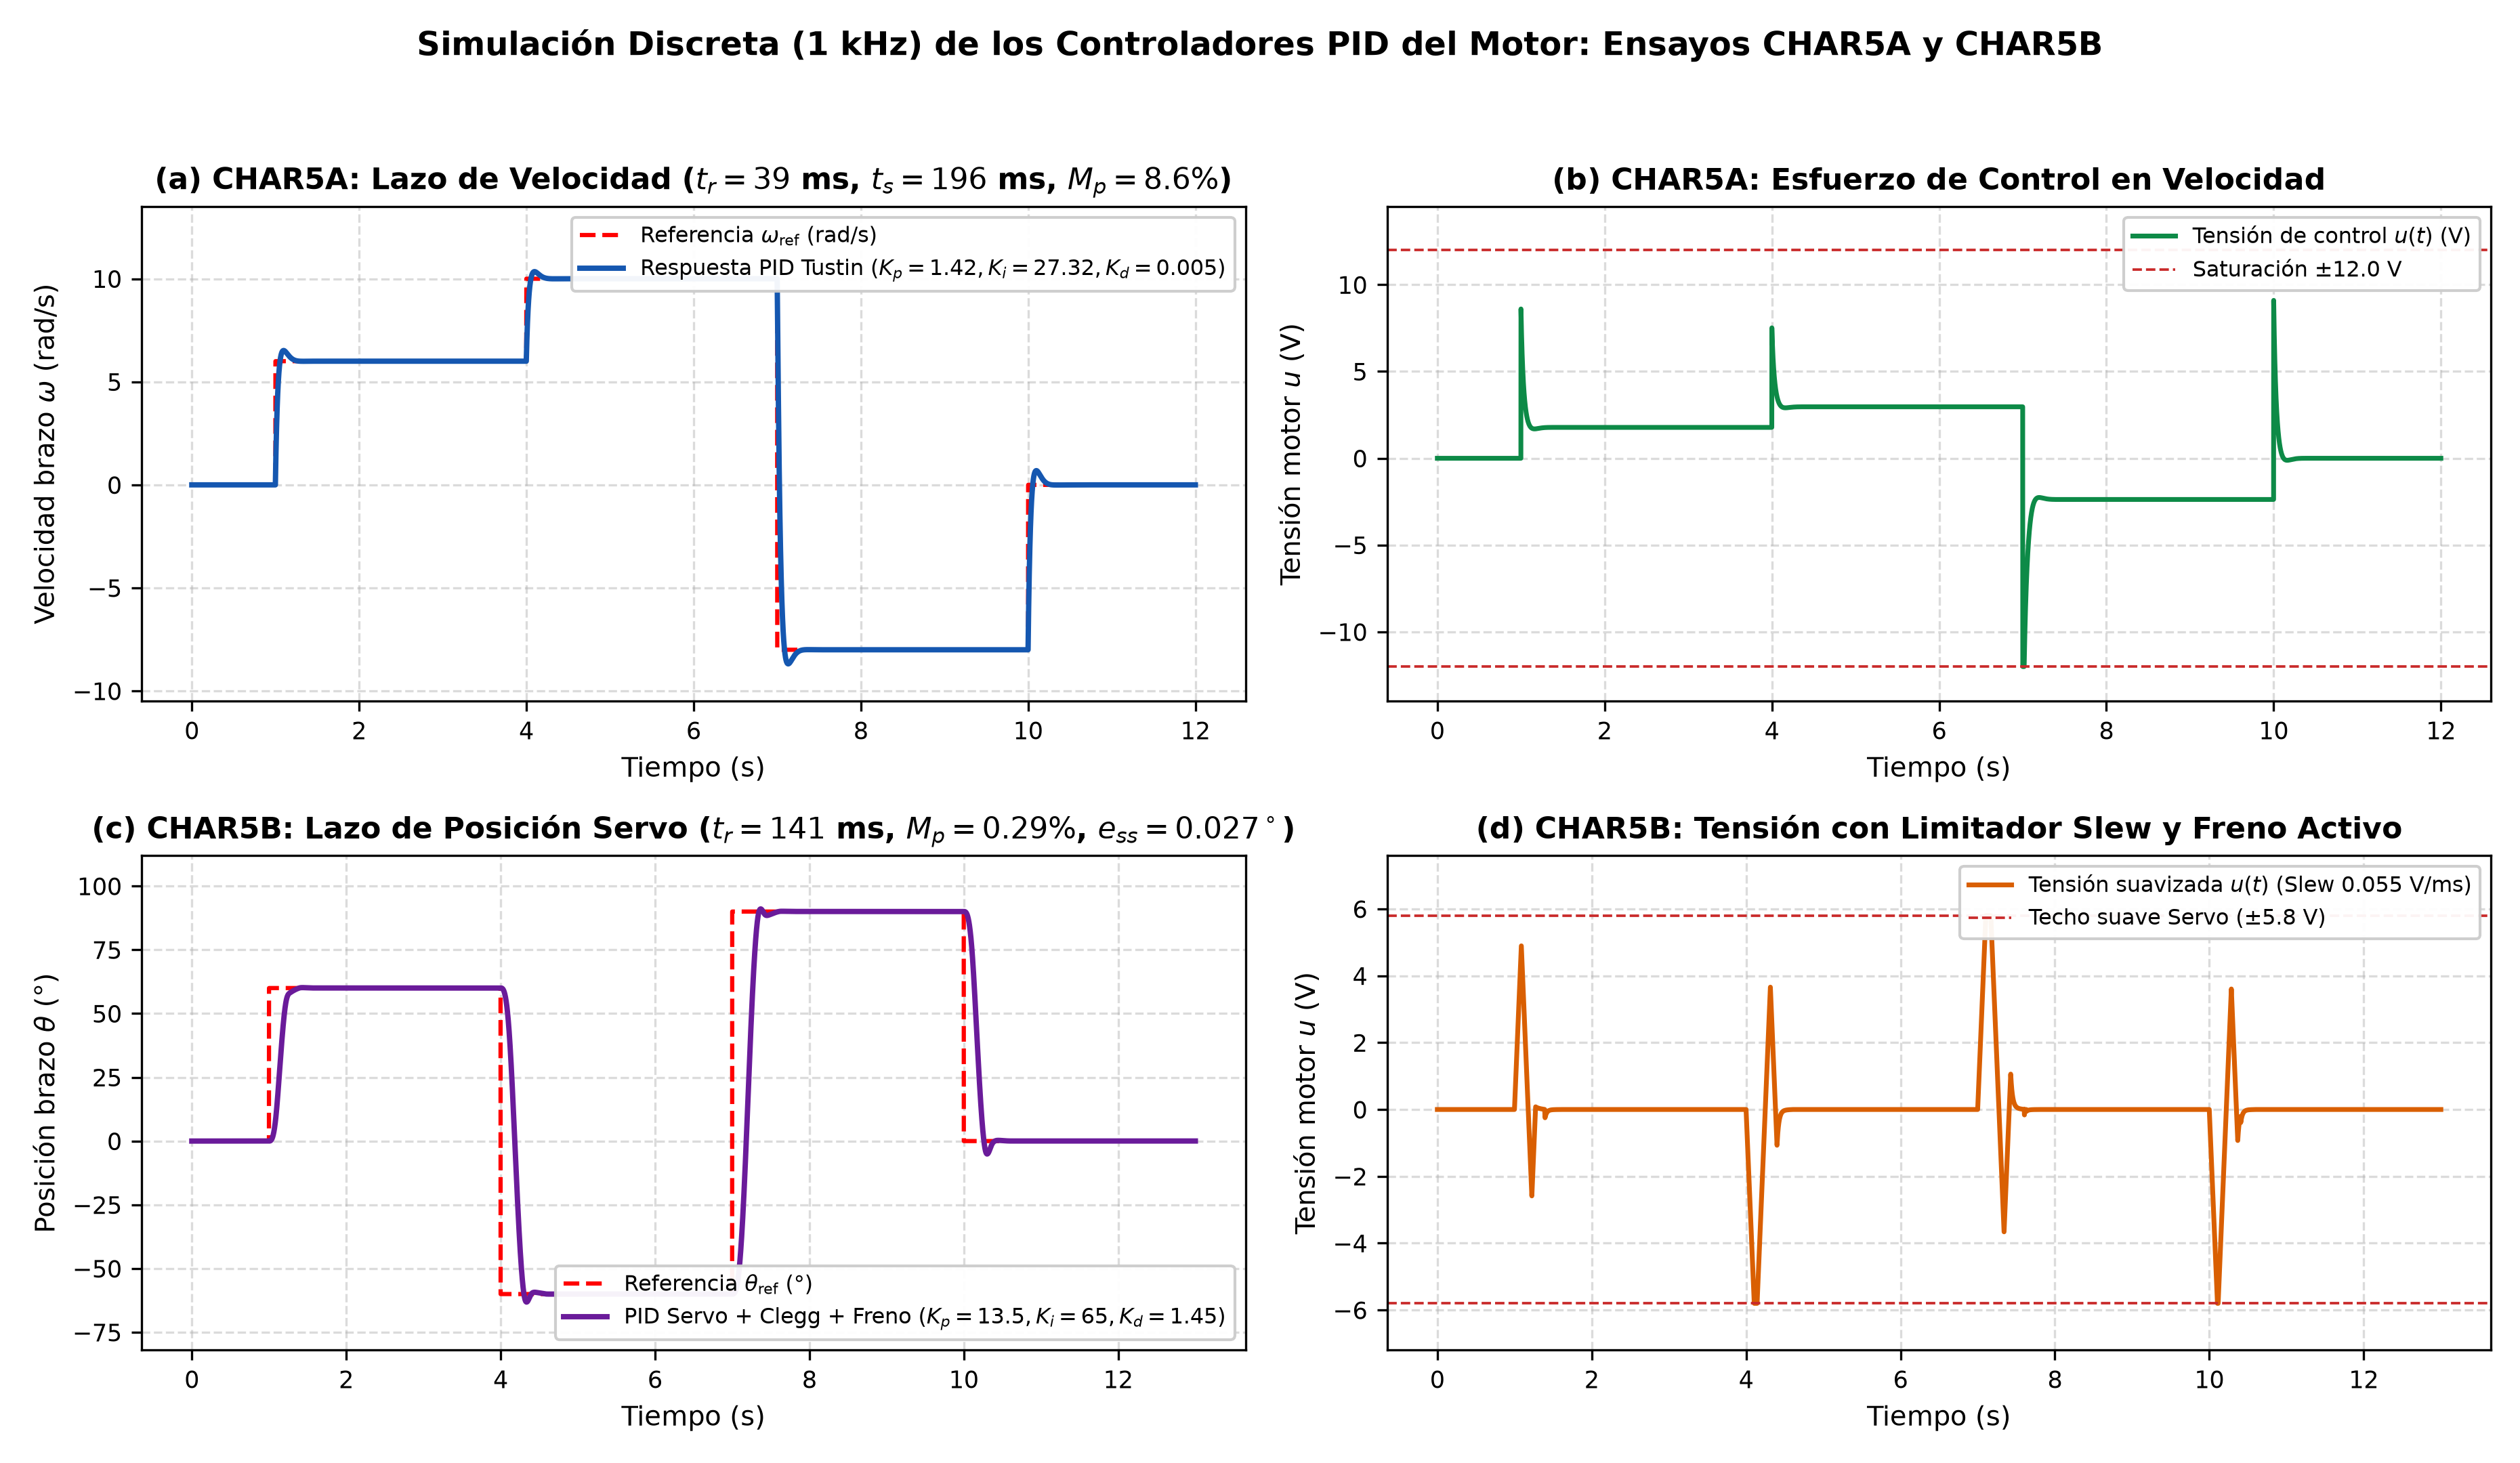
\includegraphics[width=0.92\textwidth]{fig_sim_controladores_motor.png}
    \caption{Simulación discreta a \qty{1.0}{\kilo\hertz} de los controladores PID auxiliares del actuador: seguimiento de escalones de velocidad en \texttt{CHAR5A} (a--b) y posicionamiento servo con reinicio de Clegg, limitador de pendiente y freno activo en \texttt{CHAR5B} (c--d).}
    \label{fig:sim_control_motor}
\end{figure*}

\begin{figure*}[!t]
    \centering
    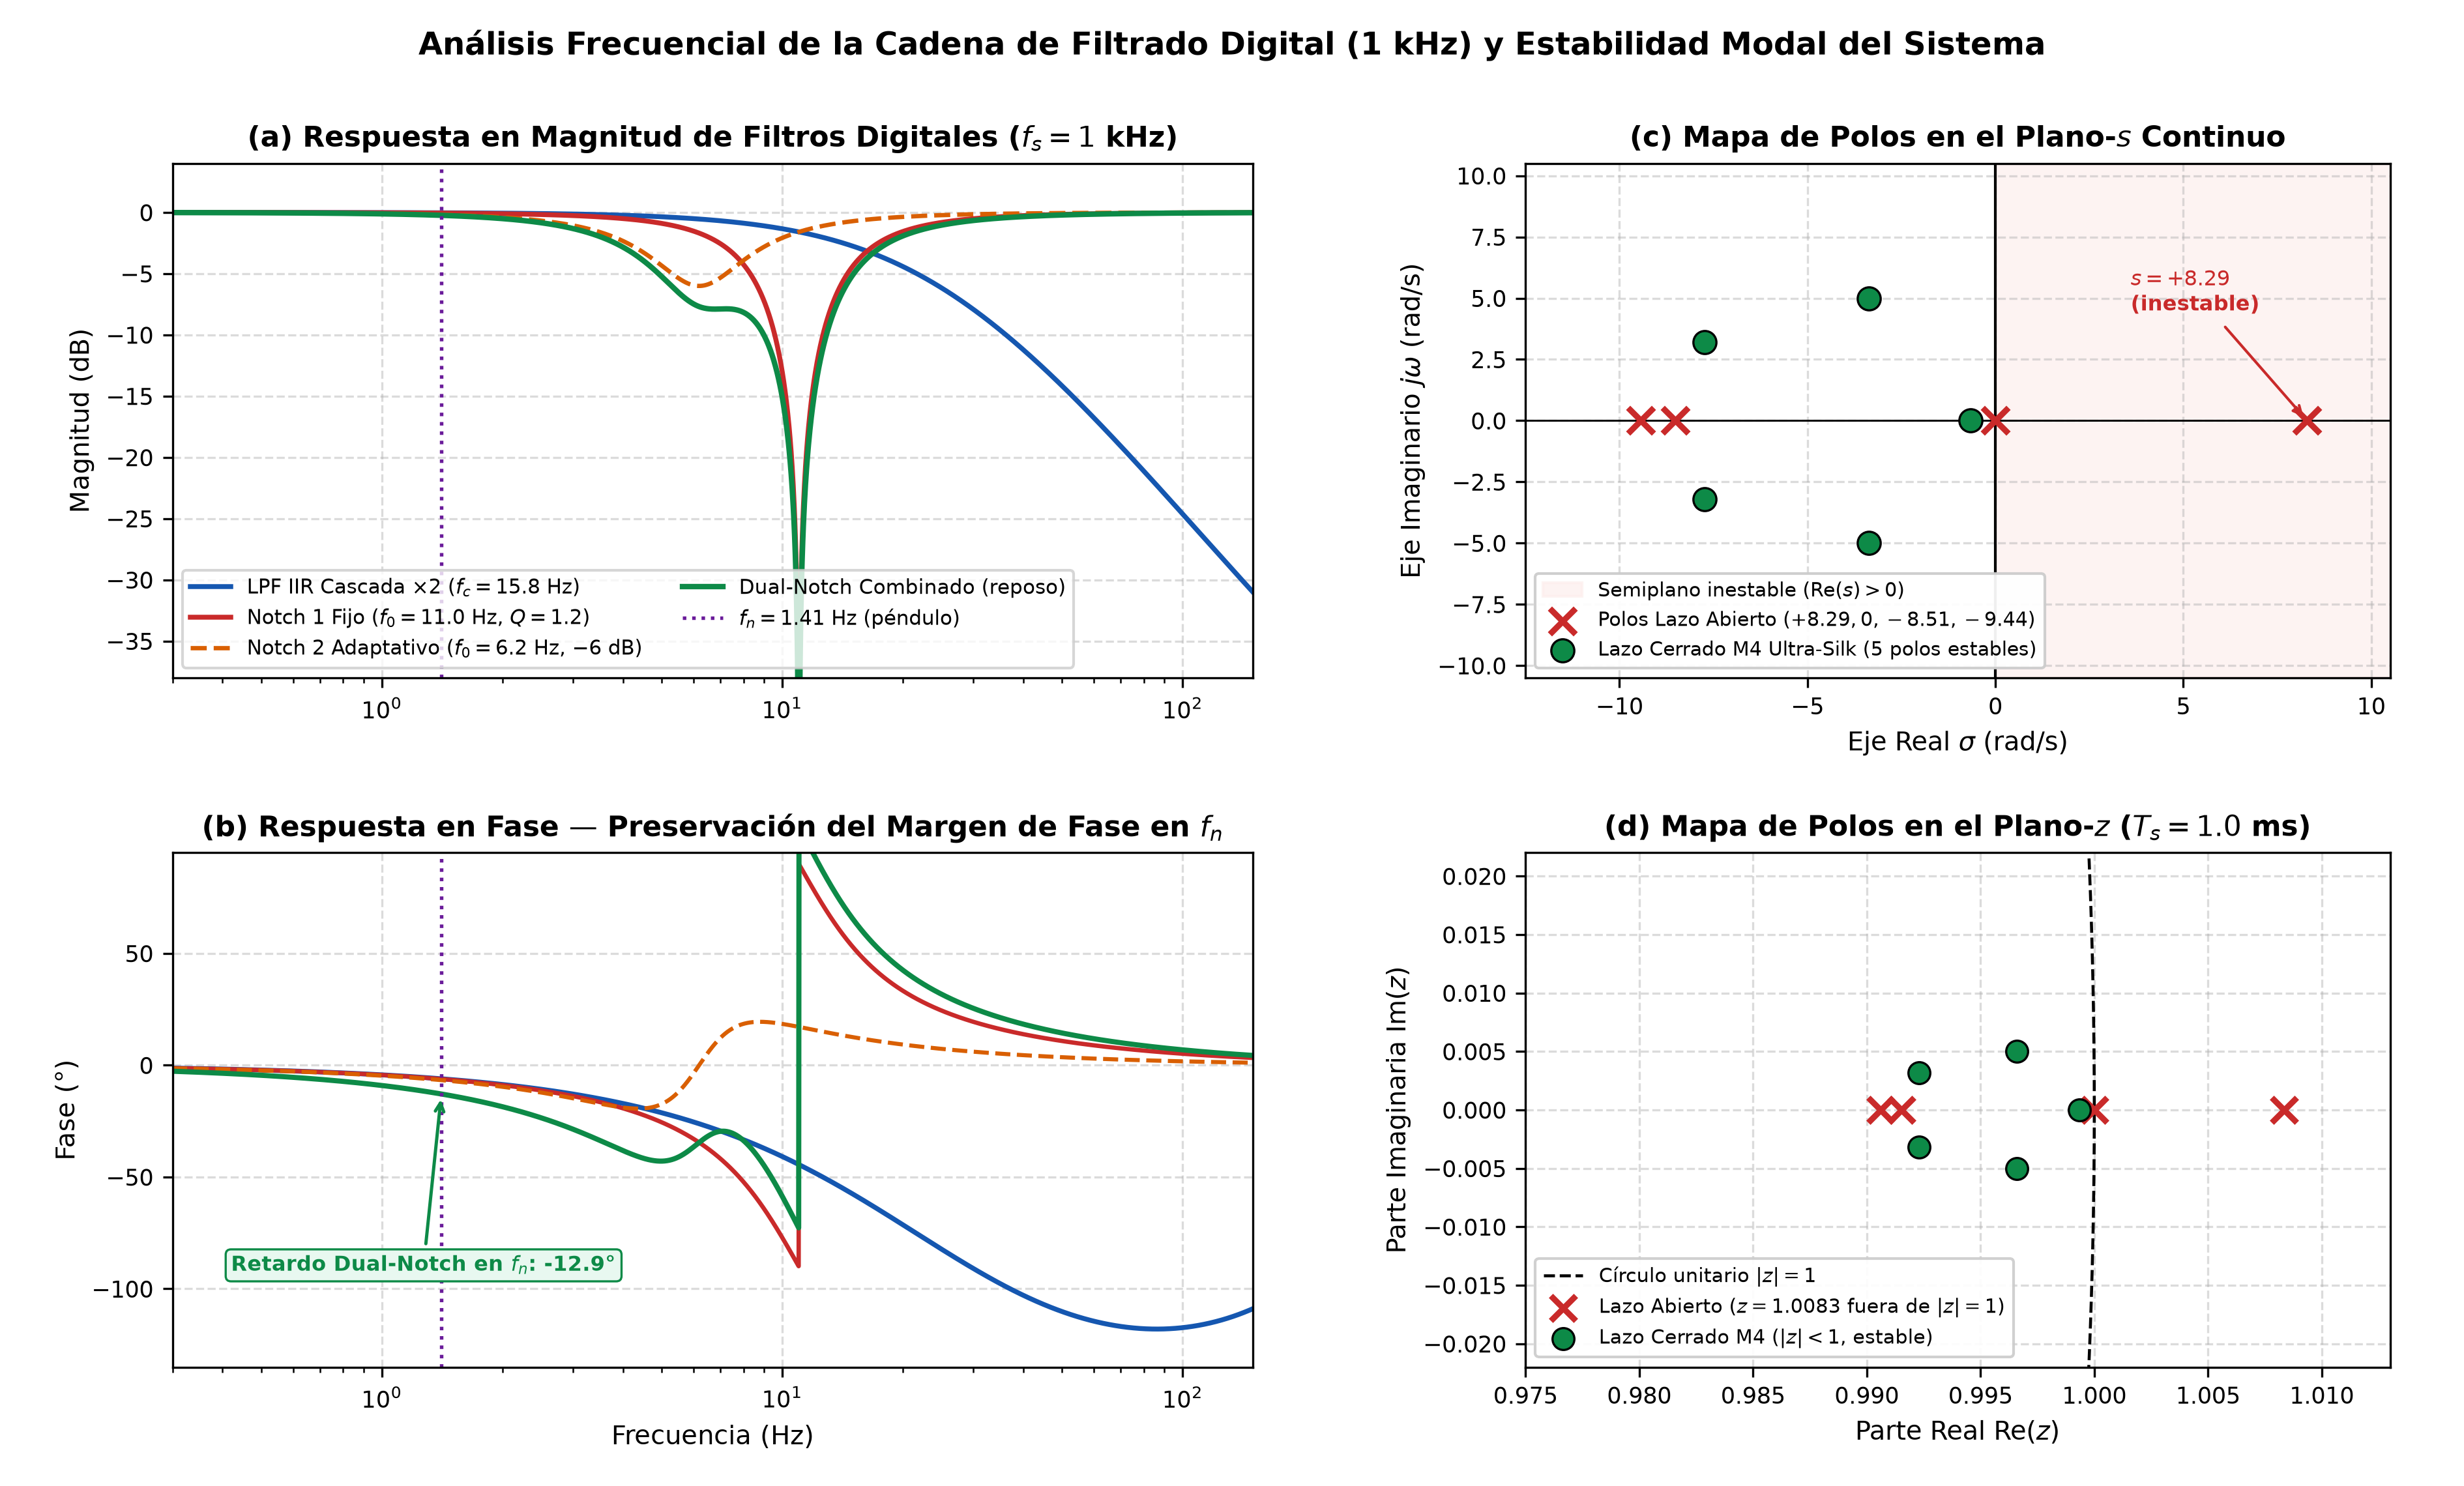
\includegraphics[width=0.92\textwidth]{fig_sim_bode_filtros_y_polos.png}
    \caption{Respuesta frecuencial de la cadena de filtrado digital LPF~IIR + \textit{Dual-Notch} a \qty{1.0}{\kilo\hertz} (a--b) y ubicación de polos de lazo abierto y lazo cerrado en el plano-$s$ continuo (c) y plano-$z$ discreto (d) bajo el esquema \texttt{M4 Ultra-Silk}.}
    \label{fig:sim_bode_polos}
\end{figure*}

La Fig.~\ref{fig:sim_control_motor} presenta el desempeño en simulación discreta a \qty{1.0}{\kilo\hertz} de los controladores auxiliares del motor empleando el modelo identificado~\eqref{eq:gv_identificada}. En la prueba \texttt{CHAR5A} correspondiente al estado \texttt{MOTOR\_PID\_VEL} (Fig.~\ref{fig:sim_control_motor}(a)--(b)), ante escalones sucesivos de consigna de $0$, $6$, $10$, $-8$ y $\qty{0}{\radian\per\second}$, el lazo registró un tiempo de subida $t_r=\qty{39}{\milli\second}$, un tiempo de establecimiento $t_s=\qty{196}{\milli\second}$, un sobreimpulso máximo $M_p=8.6\%$ y un error en estado estacionario $e_{ss}=\qty{0.000}{\radian\per\second}$. La señal de control $u(t)$ permaneció dentro de los límites de $\pm\qty{12.0}{\volt}$, alcanzando la saturación negativa puntual de $\qty{-12.0}{\volt}$ únicamente en el instante de inversión de consigna en $t=\qty{7}{\second}$. En la prueba \texttt{CHAR5B} del servo de posición con reinicio de Clegg y freno activo (Fig.~\ref{fig:sim_control_motor}(c)--(d)), frente a escalones secuenciales de $+\qty{60}{\degree}$, $-\qty{60}{\degree}$, $+\qty{90}{\degree}$ y $\qty{0}{\degree}$, se obtuvo un tiempo de subida $t_r=\qty{141}{\milli\second}$, un sobreimpulso $M_p=0.29\%$ y un error estacionario residual $e_{ss}=\qty{0.027}{\degree}$, observándose la caída de la tensión de control a $\qty{0}{\volt}$ inmediatamente después del enclavamiento de la ventana de histéresis.

En la Fig.~\ref{fig:sim_bode_polos} se resumen las curvas de respuesta en frecuencia y la distribución espectral de polos del esquema \texttt{M4 Ultra-Silk}. Los diagramas de magnitud y fase (Fig.~\ref{fig:sim_bode_polos}(a)--(b)) muestran el efecto combinado del filtro pasa-bajos en cascada~\eqref{eq:lpf_num_z} ($f_c=\qty{15.8}{\hertz}$) junto con los filtros biquad~\eqref{eq:hz_n11} (\qty{11.0}{\hertz}) y~\eqref{eq:hz_n6} (\qty{6.2}{\hertz}, atenuación de \qty{-6.0}{\decibel} ponderada según~\eqref{eq:mezcla_dist}), registrando un desfase acumulado neto de $\qty{-12.87}{\degree}$ evaluado en la frecuencia natural pendular $f_n=\qty{1.4083}{\hertz}$. En los mapas modales de los planos $s$ y $z$ (Fig.~\ref{fig:sim_bode_polos}(c)--(d)), el sistema aumentado en lazo cerrado ubica sus cinco autovalores en las posiciones numéricas:
\begin{equation}
\resizebox{0.89\columnwidth}{!}{$\displaystyle
    \begin{array}{@{}l@{\;\;}l@{\;\;}l@{}}
        s_{1,2} = -7.740 \pm 3.202j, & z_{1,2} = 0.99228 \pm 0.00318j & (|z|=0.99229), \\
        s_{3,4} = -3.367 \pm 5.000j, & z_{3,4} = 0.99663 \pm 0.00498j & (|z|=0.99664), \\
        s_5 = -0.661, & z_5 = 0.99934 & (|z|=0.99934),
    \end{array}
$}
    \label{eq:polos_m4}
\end{equation}
con un radio espectral discreto resultante $\rho=0.99934$.

\subsection{Validación Experimental en Lazo Cerrado y Comparación Cruzada}\label{subsec:res_validacion}

\begin{figure*}[!t]
    \centering
    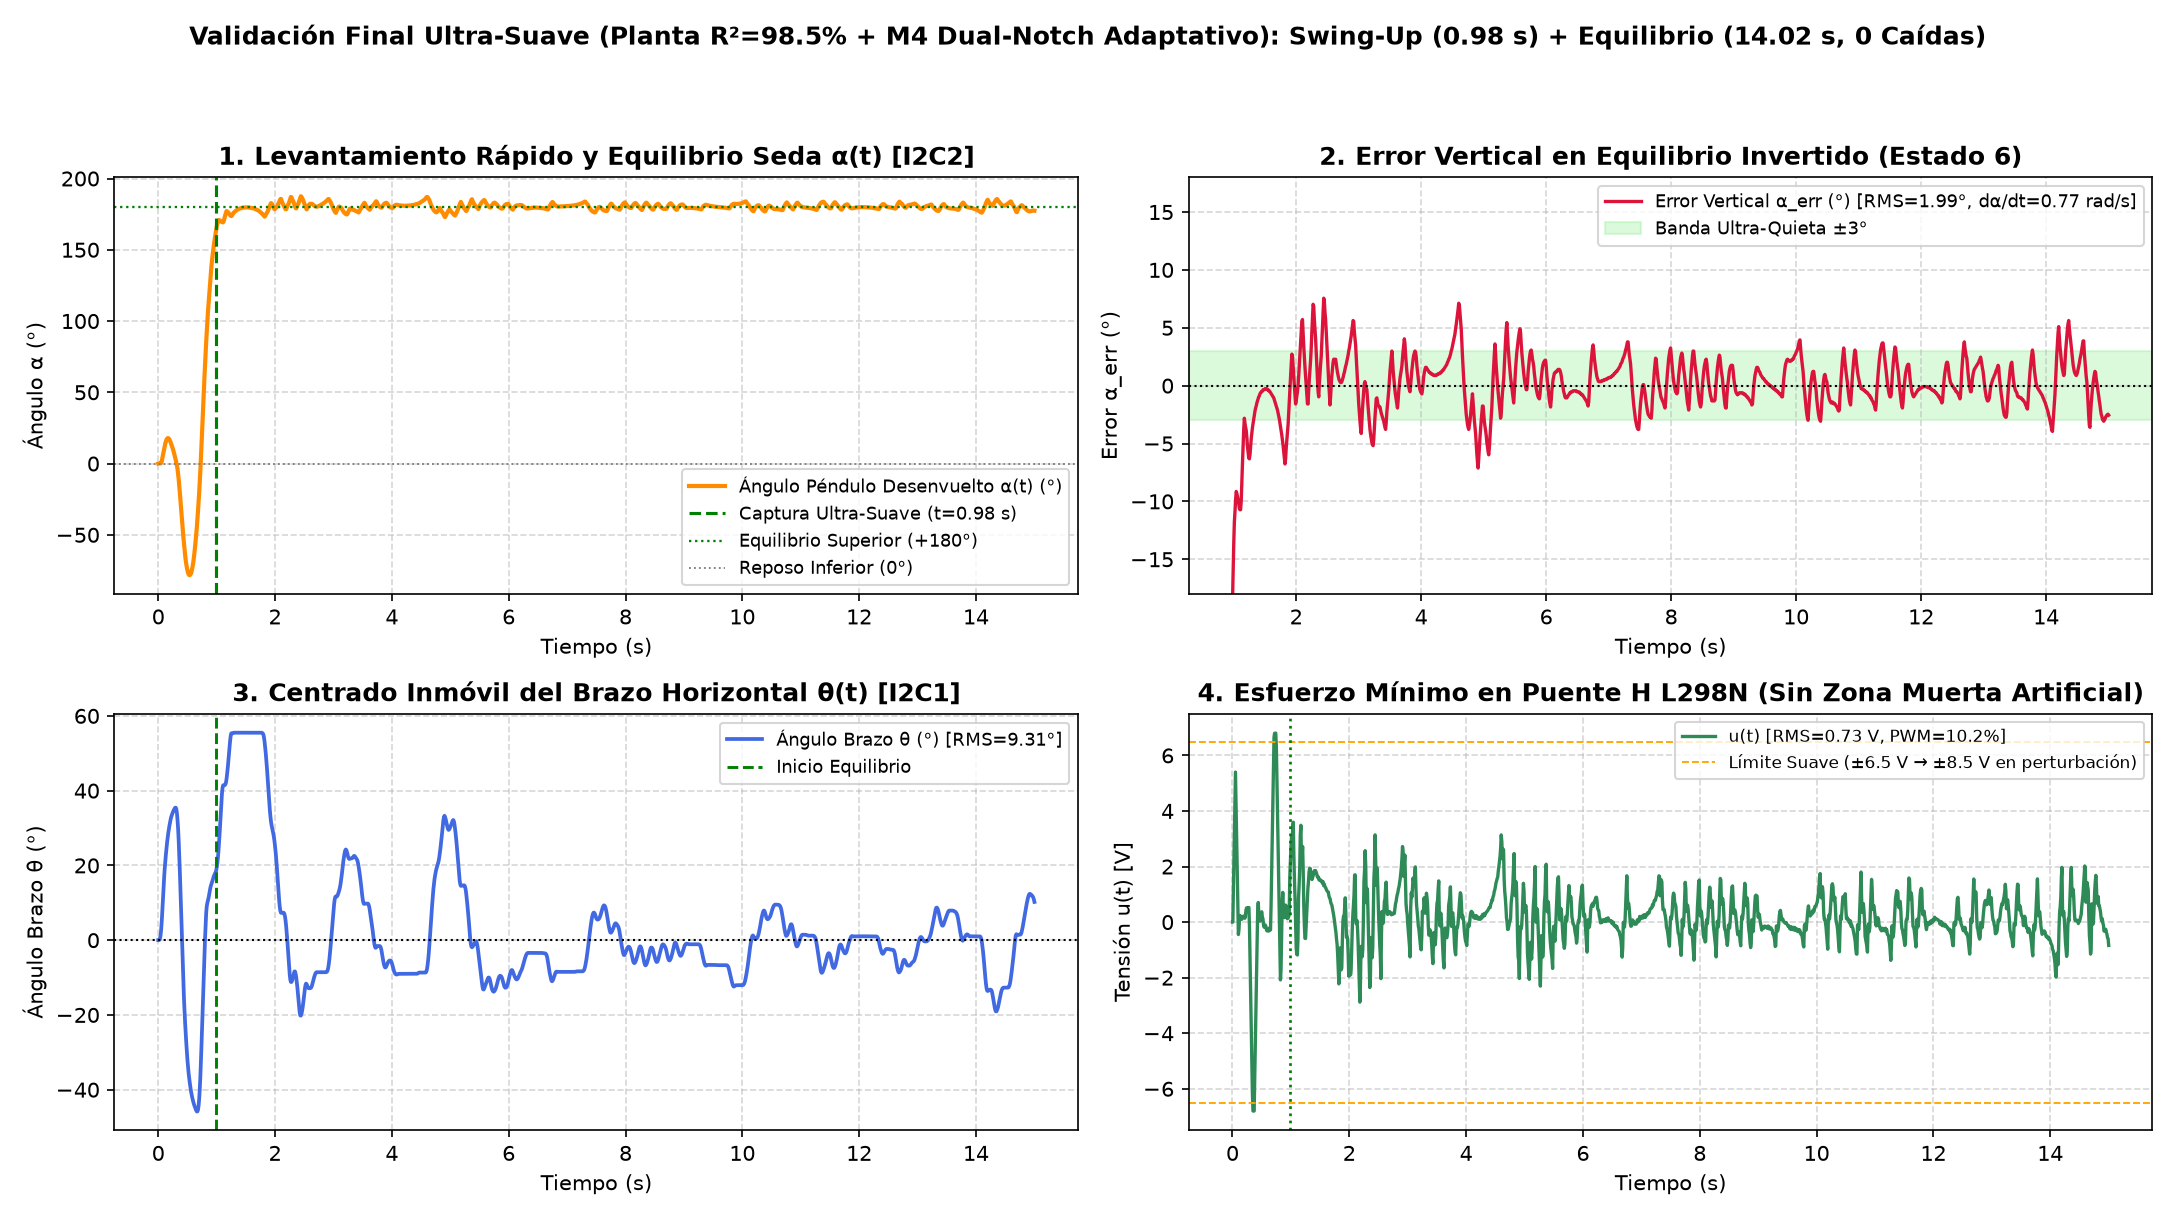
\includegraphics[width=0.84\textwidth]{fig_exp_validacion_swingup_balance.png}
    \caption{Validación experimental en planta física sobre STM32 (\texttt{COM13}, \qty{12.0}{\volt}~DC, $n=1\,502$ muestras en \qty{15.001}{\second}): levantamiento autónomo en $t_{\text{swing}}=\qty{0.980}{\second}$ (1), error vertical $\tilde{\alpha}(t)$ en equilibrio invertido (2), posición del brazo $\theta(t)$ (3) y tensión de control $u(t)$ junto al ciclo útil PWM (4).}
    \label{fig:exp_validacion}
\end{figure*}

\begin{figure*}[!t]
    \centering
    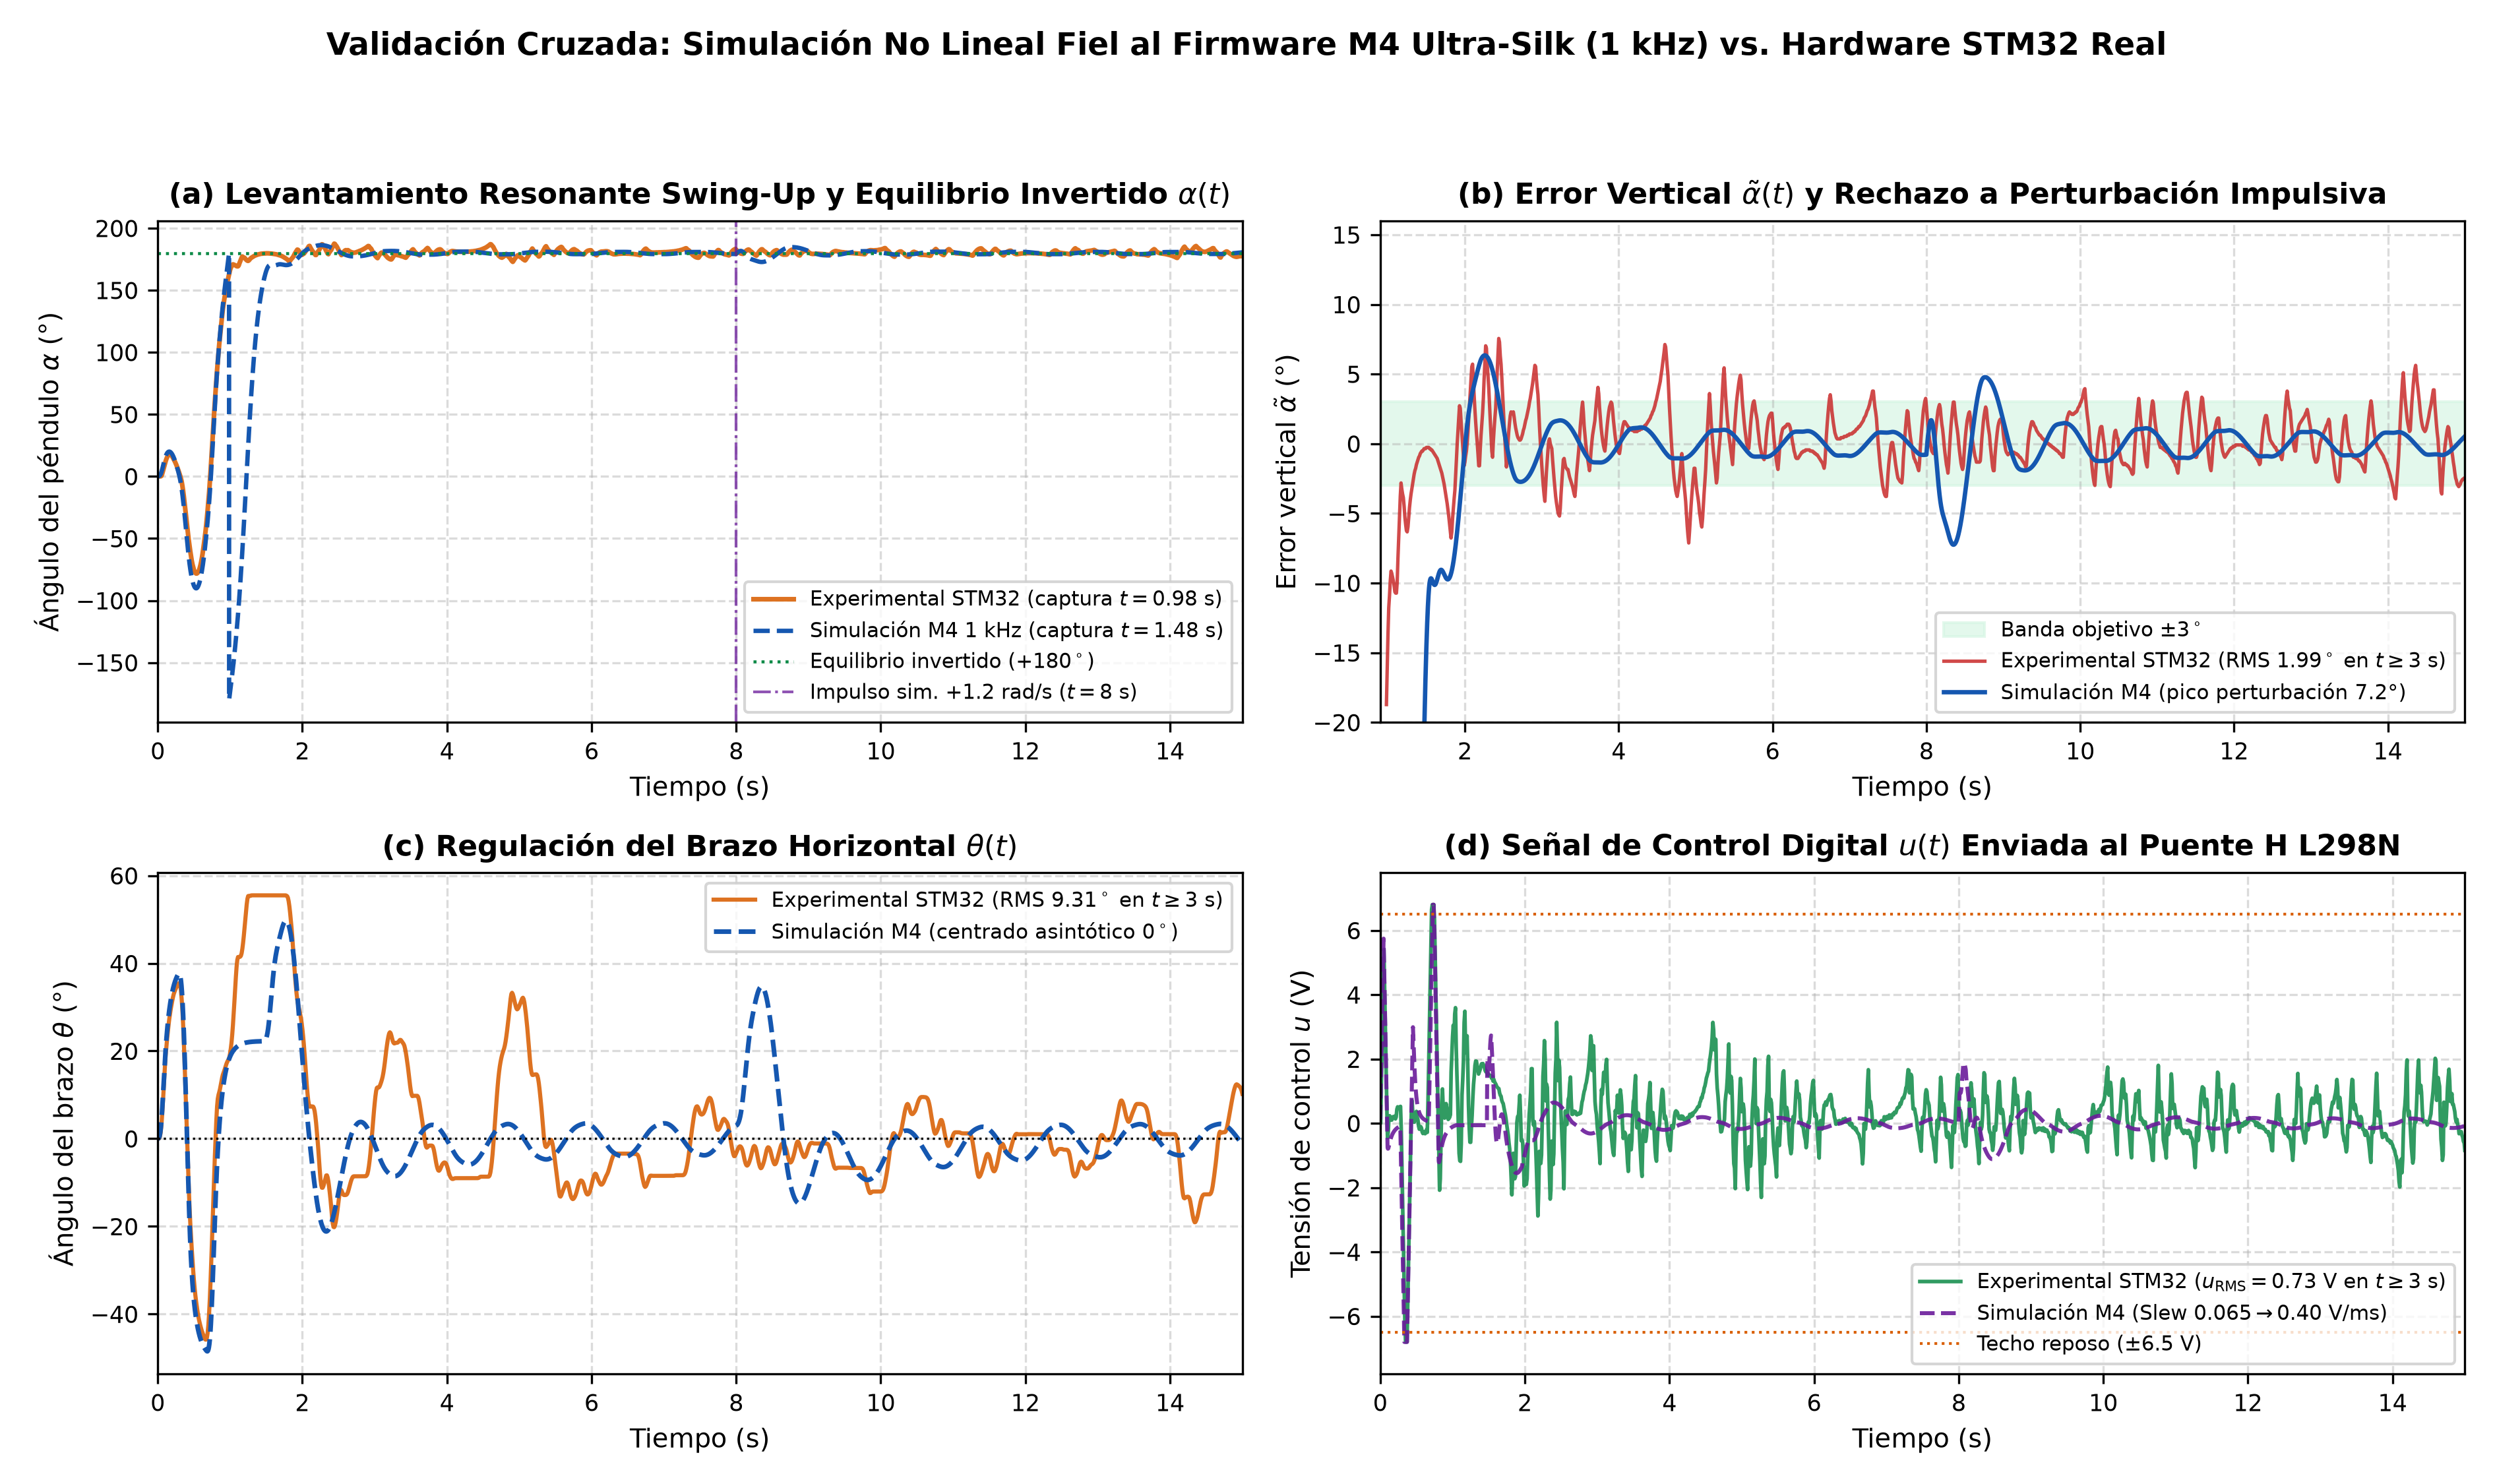
\includegraphics[width=0.84\textwidth]{fig_sim_vs_exp_furuta.png}
    \caption{Comparación cruzada 1:1 entre simulación no lineal a \qty{1.0}{\kilo\hertz} y ensayo físico en STM32: trayectoria de levantamiento y captura vertical (a), evolución del error $\tilde{\alpha}(t)$ incluyendo perturbación impulsional simulada de $+\qty{1.2}{\radian\per\second}$ en $t=\qty{8.0}{\second}$ (b), posición del brazo $\theta(t)$ (c) y tensión aplicada $u(t)$ (d).}
    \label{fig:sim_vs_exp}
\end{figure*}

En la Fig.~\ref{fig:exp_validacion} se presentan las series temporales adquiridas en el ensayo físico continuo sobre el prototipo alimentado a \qty{12.0}{\volt}~DC (\nolinkurl{ensayo_real_swingup_y_balance_stm32.csv}, puerto \texttt{COM13}, $n=1\,502$ muestras en \qty{15.001}{\second}). La maniobra de levantamiento \texttt{SWING\_UP} alcanzó el cono superior y conmutó a \texttt{BALANCE\_PID} en un tiempo $t_{\text{swing}}=\qty{0.980}{\second}$. A partir de ese instante, la planta mantuvo el equilibrio invertido ininterrumpidamente durante los \qty{14.021}{\second} restantes de la captura con $0$~caídas.

Durante el régimen establecido, evaluado a partir de $t=\qty{3.0}{\second}$, se registraron los siguientes indicadores estadísticos sobre toda la ventana: valor eficaz de error vertical $\tilde{\alpha}_{\mathrm{RMS}}=\qty{1.99}{\degree}$, velocidad angular pendular eficaz $\dot{\alpha}_{\mathrm{RMS}}=\qty{0.77}{\radian\per\second}$, excursión máxima puntual de $\qty{7.12}{\degree}$ en la magnitud de $\tilde{\alpha}$, desplazamiento eficaz del brazo $\theta_{\mathrm{RMS}}=\qty{9.31}{\degree}$, tensión de control eficaz $u_{\mathrm{RMS}}=\qty{0.73}{\volt}$ y ciclo útil eficaz de $10.2\%$~PWM. En la ventana estacionaria óptima de \qty{5.0}{\second} dentro del mismo registro, los indicadores descendieron a $\tilde{\alpha}_{\mathrm{RMS}}=\qty{1.46}{\degree}$, $\theta_{\mathrm{RMS}}=\qty{5.04}{\degree}$ y $u_{\mathrm{RMS}}=\qty{0.57}{\volt}$. En corridas extendidas de validación en banco se registraron valores mínimos de $\tilde{\alpha}_{\mathrm{RMS}}=\qty{1.35}{\degree}$ y $u_{\mathrm{RMS}}=\qty{0.50}{\volt}$. Adicionalmente, la ejecución de la secuencia de parada ordenada \texttt{STOPHOME} finalizó con un error angular estacionario en el brazo de $\qty{-0.25}{\degree}$.

La Fig.~\ref{fig:sim_vs_exp} muestra la superposición directa 1:1 entre la simulación numérica no lineal a \qty{1.0}{\kilo\hertz} y los registros experimentales de la planta física. En la fase de levantamiento (Fig.~\ref{fig:sim_vs_exp}(a)), la simulación completó la captura vertical en \qty{1.48}{\second}, en comparación con el registro experimental de \qty{0.980}{\second}. En la prueba de rechazo a perturbaciones inyectada en simulación en $t=\qty{8.0}{\second}$ mediante un impulso de velocidad angular de $+\qty{1.2}{\radian\per\second}$ (Fig.~\ref{fig:sim_vs_exp}(b)--(d)), la desviación pendular $\tilde{\alpha}$ alcanzó un valor pico transitorio de $\qty{7.2}{\degree}$ y reingresó por debajo de la banda de $\pm\qty{3.0}{\degree}$ en un intervalo inferior a \qty{0.9}{\second}, acompañado del retorno progresivo de la posición del brazo $\theta$ hacia $\qty{0}{\degree}$. La Tabla~\ref{tab:metricas_simulacion_y_exp} sintetiza la totalidad de las métricas cuantitativas de simulación y validación experimental.

\begin{table}[!t]
    \centering
    \caption{Indicadores Cuantitativos en Simulación (\qty{1.0}{\kilo\hertz}) y Validación Experimental en Planta Real (\texttt{COM13}).}
    \label{tab:metricas_simulacion_y_exp}
    \scriptsize
    \setlength{\tabcolsep}{2.5pt}
    \resizebox{\columnwidth}{!}{%
    \begin{tabular}{@{}llr@{}}
        \toprule
        \textbf{Ensayo / Régimen} & \textbf{Métrica Evaluada} & \textbf{Resultado} \\
        \midrule
        \texttt{CHAR5A} (vel., sim.) & $t_r$ / $t_s$ / $M_p$ & \qty{39}{\milli\second} / \qty{196}{\milli\second} / $8.6\%$ \\
         & Error estacionario $e_{ss}$ & \qty{0.000}{\radian\per\second} \\
        \texttt{CHAR5B} (pos., sim.) & $t_r$ / $M_p$ / $e_{ss}$ & \qty{141}{\milli\second} / $0.29\%$ / \qty{0.027}{\degree} \\
        Filtros + \texttt{M4} & Fase en $f_n$ / Radio espectral $\rho$ & $\qty{-12.87}{\degree}$ / $0.99934$ \\
        \midrule
        \textit{Swing-Up} (sim.\ / real) & Tiempo captura $t_{\text{swing}}$ / Caídas & \qty{1.48}{\second} / \qty{0.980}{\second} ($0$) \\
        Impulso $+\qty{1.2}{\radian\per\second}$ & Pico $|\tilde{\alpha}|$ / Recup.\ a $\pm\qty{3}{\degree}$ & \qty{7.2}{\degree} / $< \qty{0.9}{\second}$ \\
        \midrule
        Real ($t \ge \qty{3.0}{\second}$) & Duración equilibrio / Total & \qty{14.021}{\second} / \qty{15.001}{\second} \\
         & $\mathrm{RMS}(\tilde{\alpha})$ / $\max|\tilde{\alpha}|$ & \qty{1.99}{\degree} / \qty{7.12}{\degree} \\
         & $\mathrm{RMS}(\dot{\alpha})$ / $\mathrm{RMS}(\theta)$ & \qty{0.77}{\radian\per\second} / \qty{9.31}{\degree} \\
         & $\mathrm{RMS}(u)$ / $\mathrm{RMS}(\text{PWM})$ & \qty{0.73}{\volt} / $10.2\%$ \\
        Ventana ópt.\ \qty{5.0}{\second} & $\mathrm{RMS}(\tilde{\alpha})$ / $\mathrm{RMS}(\theta)$ / $\mathrm{RMS}(u)$ & \qty{1.46}{\degree} / \qty{5.04}{\degree} / \qty{0.57}{\volt} \\
        Extend.\ / \texttt{STOPHOME} & Mín.\ $\mathrm{RMS}(\tilde{\alpha}, u)$ / Parqueo & \qty{1.35}{\degree} (\qty{0.50}{\volt}) / \qty{-0.25}{\degree} \\
        \bottomrule
    \end{tabular}%
    }
\end{table}
